\chapter{Criptografía usada en el proyecto.}\label{cap:criptografia}
\markboth{CAPÍTULO \ref{cap:criptografia}. CRIPTOGRAFÍA USADA EN EL PROYECTO.}{}

En la sección \ref{lbl:criptografia} del capítulo \ref{cap:conocimientos} hemos hecho una breve introducción a la criptografía de clave pública, a continuación vamos a explicarla con más extensión y los usos que le hemos dado en el proyecto.

Toda la criptografía que hemos usado es criptografía de clave pública, y en concreto el criptosistema llamado RSA. En el proyecto se ha usado la criptografía para firmar digitalmente, no para cifrar los mensajes.

\section{RSA.}

RSA se basa en la idea de que multiplicar dos números enteros primos, pero muy difícil sabiendo el resultado de la multiplicación averiguar dichos dos números.

El proceso de generación de las claves se va a explicar a continuación:
\begin{itemize}

	\item Se eligen dos números primos grandes que llamaremos \textbf{p} y \textbf{q}, dichos números se multiplican y obtenemos \textbf{n}, $n = p \cdot q$, dicho valor de $n$ es el que se usa como módulo de la clave pública y privada. 

	\item Calculamos $\varphi(n)$ de la siguiente forma $\varphi(n)=(p-1)\cdot(q-1)$, donde $\varphi(n)$ es la función $\varphi$ de Euler.

	\item Se elige un entero positivo $e$ menor que $\varphi(n)$ y que sea coprimo con $\varphi(n)$. El valor $e$ es el exponente de la clave pública.
	
	\item Se busca un valor $d$ que satisfaga la congruencia $d=e^{-1}\,mod\,\varphi(n)$. Este valor se suele calcular con el algoritmo de Euclides extendido y el valor $d$ es el exponente para la clave privada. 
\end{itemize}

La clave pública será $(n,e)$ y la clave privada será $(n,d)$.

El proceso de cifrado y descifrado es el siguiente:

\begin{itemize}
	\item \textbf{Cifrado:} el receptor (Alice) envía su clave pública $(n,e)$ al emisor (Bob) y guarda la clave privada, $(n,d)$, en secreto, a partir de este momento Alice usando la clave pública de Bob puede comunicarse seguramente. El mensaje que Bob quiere enviar a Alice será $M$. Bob primero convierte $M$ en un número menor que $n$, y que sea de una forma reversible de forma que sabiendo $n$ podamos volver a conseguir $M$. Acto seguido calcula $c$ de esta forma, $c\equiv m^e\,(mod\,n)$. Bob mandaría $c$ a Alice y la comunicación finalizaría.
	
	\item \textbf{Descifrado:} Alice empezará el proceso para recuperar $m$ a partir de $c$ y $d$. $m\equiv c^d\,(mod\,n)$, una vez ha calculado $m$ puede conseguir $M$.

\end{itemize}

El proceso de descifrado funciona porque $c^d=(m^e)^d\equiv m^{ed}\, (mod\, n)$ y hemos elegido $d$ y $e$ de forma que $e\cdot d =1+k\cdot\varphi(n)$, se cumple que $ m^{ed}\cdot m^{1+k\cdot\varphi(n)} = m(m^{\varphi(n)})^k = m\, (mod\, n)$, esta última congruencia se obtiene directamente del teorema de Euler cuando $m$ y $n$ son coprimos.

Un ejemplo de cifrado y descifrado mediante el algoritmo RSA es el siguiente:

\begin{itemize}

\item Elegimos $p=61$, $q=53$. Podemos observar que ambos son primos. Se ha elegido para el ejemplo unos valores pequeños para que podamos hacer los cálculos con facilidad.

\item Calculamos $n=p\cdot q= 3233$.

\item Elegimos $e=17$ y $d=2753$, como exponente público $e$ y como exponente privado $d$. La clave pública quedaría como $(17, 3233)$ y la clave privada sería $(2753, 3233)$.

\item La función de cifrado quedaría como la siguiente: $\mbox{encrypt}(m) = m^e \,mod(n) = m^{17}\,mod(3233)$, donde $m$ es el texto sin cifrar. Imaginemos que $m=123$, luego los cálculos quedarían, $\mbox{encrypt(123)} = 123^{17}\,mod(3233) = 855$.

\item La función de descifrado sería: $\mbox{decrypt(c)} = c^d\,mod(n) = c^{2753}\,mod(3233)$, donde $c$ es el mensaje cifrado. Usando la función para descifrar $c=855$ obtenemos lo siguiente: $\mbox{decrypt(855)} = 855^{2753}\,mod(3233) = 123$.

\end{itemize}

Podemos observar que hemos conseguido cifrar y descifrar de forma segura usando dos claves diferentes y una de ellas es pública.

Una de las característica del algoritmo RSA es que permite la verificación de la veracidad de documentos mediante un proceso que se llama firma digital. Con ello no garantizamos que un atacante no pueda leer el mensaje, ya que no nos importa, pero si podemos garantizar que dicho mensaje no ha sido modificado. 

La forma de realizar la firma es la siguiente, en vez de firmar todo el documento, que sería un gran problema ya que estos algoritmos son muy lentos, Alice genera un hash del documento con una longitud fija (128 o 256 bits) y se firma dicho hash con su firma privada. Una función hash es una función matemática que para una entrada devuelve un valor único, por lo que podemos garantizar que un documento sólo va a devolver un valor numérico único y si modificamos algo del documento ese valor se alterará. Acto seguido se envía el valor de la función hash firmado junto con el documento original. Cuando Bob recibe el mensaje lo único que tiene que hacer es volver a generar el hash del documento de la misma forma que lo hizo Alice y usando la clave pública de Alice descifrar el hash firmado. Si ambos valores son iguales podemos garantizar que el mensaje es el original que Alice quería enviar.

En el proyecto hemos usado librerías que proporciona Java en su API \lstinline{java.security.*}. En dicha librería, como veremos en la sección \ref{cap:javasecurity} con más profundidad, se nos proporcionan todas las utilidades para manejo y creación de claves públicas y privadas, keystores, certificados de clave pública, funciones hash, algoritmos como RSA o DSA y algoritmos de cifrados simétricos, etc. 

Generalmente cuando se intercambian las claves no se pasan los números en un par como hemos hecho anteriormente ya que los números primos no son de dos dígitos son números primos muy grandes, se usan contenedores de certificados de claves en los que van incluidos ambas claves o sólo la pública, además de más datos como entidades que verifican que el certificado es real. Uno de los grandes problemas que tiene la criptografía de clave pública es que cualquiera puede generar un certificado y decir que es otra persona, por lo que se necesita de entidades ajenas y que no tengan ningún compromiso con ninguna de las partes. Esto es lo que se llama una PKI (Public-Key Infrastructure).

\section{Public-Key Infrastructure.}

Una PKI es una combinación de hardware, software, políticas y procedimientos de seguridad que garantizan las operaciones de cifrado, firma digital y el no repudio de las transacciones electrónicas y que se encargan de crear, almacenar, distribuir, usar y revocar los certificados digitales usados por empresas y particulares para garantizar las comunicaciones electrónicas. Esto se puede garantizar gracias a autoridades de certificación, que son empresas o entidades públicas que garantizan todo lo anterior.

Hay varias entidades dentro del sistema como puede ser una CA (Certificate Authority) que es la entidad que firma todos los certificados, sólo se usa para auto firmarse el certificado de ella y para firmar a las entidades certificadoras subordinadas, si este nodo del sistema es comprometido, toda la estructura caerá. Las autoridades subordinadas son las encargadas de certificar digitalmente a un usuario y garantizar que el usuario es real y de verdad es quien dice ser.  Las VA (Validation Authority) es la autoridad que se encarga de comprobar el estado del certificado emitido, si es válido o está revocado. Para asegurar que cada clave pública es única y pertenece a un usuario real se usa una RA (Registration Authority), la cual se encarga de verificarlo. Hay otra entidad importante que son los repositorios para almacén de certificados y los repositorios de listas de revocación de certificados. La lista de revocación es un componente muy importante de la PKI, ya que en dicha lista están los certificados revocados antes del tiempo indicado dentro del certificado. También suelen incluir TSA (TimeStamp Authority) que es la encargada de certificar que la operación fue realizada en tiempo en concreto.

\begin{figure}
  \centering
    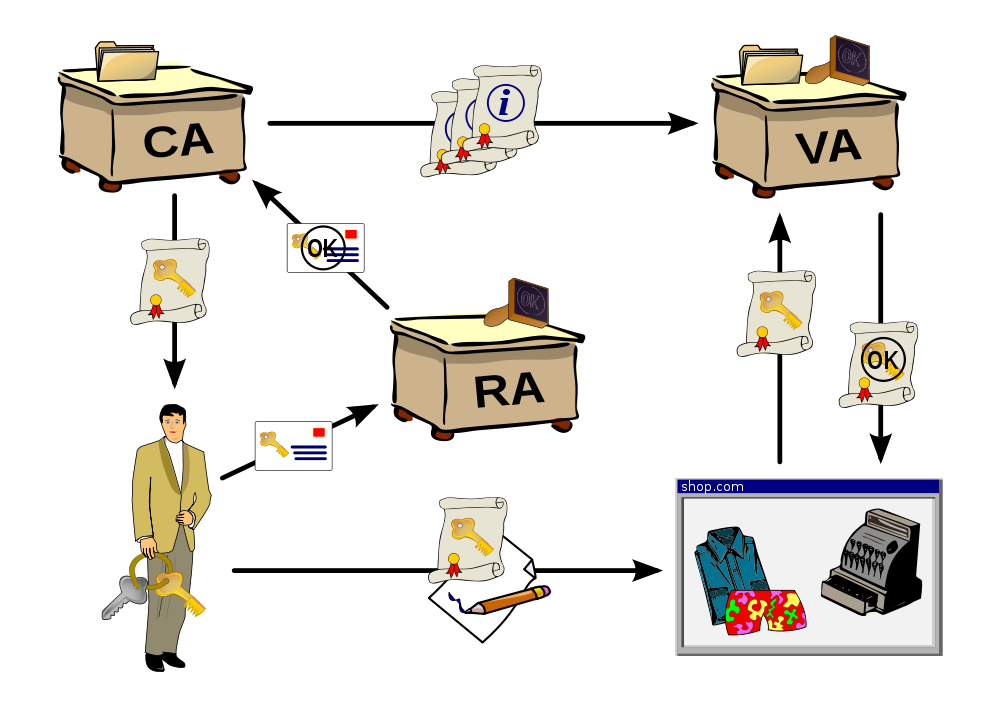
\includegraphics[scale=0.3]{./Criptografia/imagenes/esquemaPKI.png}
  \caption{Estructura genérica de una PKI.}
  \label{fig:esquemaPKI}
\end{figure} 

En la figura~\ref{fig:esquemaPKI} podemos ver todas las autoridades y sus relaciones que hemos explicado anteriormente.

En España tenemos dos PKI, una creada por la FNMT y otra creada por la Policía Nacional para dotar al DNIe de todos los certificados necesarios para que se pueda verificar la veracidad de un usuario de forma telemática. Tiene una estructura en la que hay una CA principal que está en la raíz y de ella cuelgan tres autoridades certificadoras subordinadas las emiten los certificados que se usan en el DNIe. La VA serían las comisarías donde se consigue el DNIe, donde se tiene que certificar que eres esa persona para conseguir el DNIe. En la figura \ref{fig:pkiDnie} se puede ver la estructura.

\begin{figure}
  \centering
    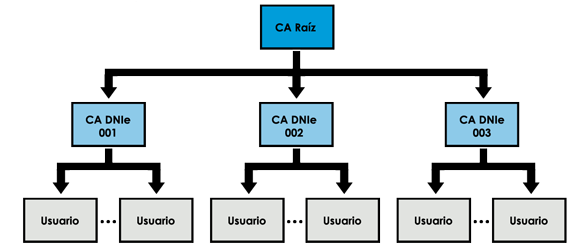
\includegraphics[scale=0.9]{./Criptografia/imagenes/pkiDnie.png}
  \caption{Jerarquía de la PKI del DNIe.}
  \label{fig:pkiDnie}
\end{figure} 

Una PKI puede garantizar la veracidad de la autentificación frente a otros usuarios y proporciona métodos para conseguir certificados de identidad de otros usuarios para firmar digitalmente, cifrar y descifrar. En toda operación hay tres pasos principales, el primero es el inicio de un usuario de la operación, el segundo un sistema de servidores que dan fe de que la operación ha ocurrido y garantizan la veracidad, como puede ser servidores de timestamp, la autoridad de certificación y la autoridad de registro, el tercer paso es el receptor recibe los datos firmados o cifrados y puede garantizar la veracidad de los documentos.

La tecnología PKI se puede usar para los siguientes casos, autentificación de usuarios y sistemas, identificación del interlocutor, cifrado de datos digitales, firmado digital de datos, tales como documentos, software, etc, asegurar comunicaciones y garantía de no repudio.

Existen varios tipos de certificados entre los que podemos encontrar certificados de tipo personal, que acredita la identidad del titular, un certificado de pertenencia a una empresa, que además de garantizar la identidad garantiza la empresa para la que trabaja, certificado de representante, que acredita los poderes que tiene dicho usuario sobre la empresa, certificado de servidor seguro, que utilizan los servidores para asegurar las conexiones con sus clientes, certificados de firma de código para garantizar que los cambios realizados en el código son legítimos y muchos otros tipos.

En el ámbito de servidores y sistemas informáticos hay varias PKI importantes como Verisign\footnote{ Se puede ver toda la información en su página web: \url{http://www.verisign.com/}} o Comodo\footnote{ Se puede ver toda la información en su página web: \url{http://www.comodo.com}}.  


En el proyecto hemos usado certificados generados por una CA imaginaria, en el anexo~\ref{cap:anexoB} podemos ver como generar certificados para poder hacer las pruebas, pero si el proyecto se realizara podría ser fácilmente extensible con una PKI propia de la Universidad de Málaga o con cualquiera que dote a todo el sistema de validez legal en España.

\section{Criptografía en Java.}\label{cap:javasecurity}

Como ya hemos dicho Java dota de una API llamada \lstinline{java.security}, donde proporciona todo tipo de algoritmos para la realización de funciones hash, firmas digitales, cifrados, generación de números aleatorios, etc. En \url{http://docs.oracle.com/javase/6/docs/technotes/guides/security/} podemos encontrar la documentación necesaria sobre todos los métodos de cifrado o firmado que proporciona la API.

El paquete \lstinline{java.security.*} proporciona diferentes clases que vamos a explicar a continuación:



\textbf{MessageDigest:} es la clase que proporciona todos los mecanismos para realizar funciones hash. La generación de un hash se puede observar en la figura~\ref{fig:messageDigest}. 

\begin{figure}[h]
  \centering
    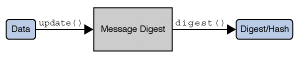
\includegraphics[scale=1.3]{./Criptografia/imagenes/messageDigest.png}
  \caption{Uso de la clase MessageDigest.}
  \label{fig:messageDigest}
\end{figure} 

La forma de uso es la siguiente, primero se genera un objeto del tipo \lstinline{MessageDigest}, el objeto se inicializa con la función \lstinline{getInstance()} de la fábrica de métodos estáticos que proporciona la clase, acto seguido se usa el método \lstinline{update()} para añadir los byte del mensaje al que queremos realizar la función hash y seguidamente usamos la función \lstinline{digest()} que devuelve el hash del mensaje que hemos introducido con el método \lstinline{update()}. Un ejemplo de esto se puede ver en el código que se muestra a continuación.

\begin{lstlisting}[style=Java] 
MessageDigest md = MessageDigest.getInstance("SHA");
md.update(toChapter1);
byte[] toChapter1Digest = tc1.digest();
\end{lstlisting}

\textbf{Signature:} es la clase que proporciona todos los métodos de firmado mediante algoritmos RSA o DSA. En la figura \ref{fig:signature} podemos ver el modo de uso. Para usarlo primero hay que poseer una clave (Key), puede ser una clave pública o privada y dependiendo de cual poseamos podemos firmar o verificar una firma. En el proyecto hemos usado la instancia \lstinline{SHA1withRSA}.

\begin{figure}[h]
  \centering
    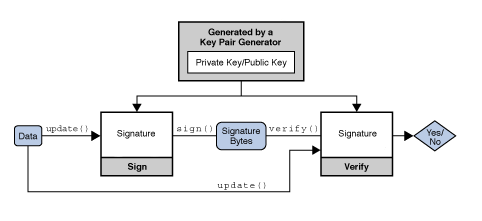
\includegraphics[scale=0.8]{./Criptografia/imagenes/signature.png}
  \caption{Modo de uso de la clase Signature.}
  \label{fig:signature}
\end{figure} 

El uso es muy parecido a la clase de \lstinline{MessageDigest}, lo primero es crear un objeto usando la función \lstinline{getInstance()} de la fábrica de clases con la instancia que queramos usar, acto seguido usamos el método \lstinline{initSign(Key)} con la que añadimos la clave al proceso, a continuación usamos el método \lstinline{update()} y añadimos los datos que queremos firmar o verificar. Si lo que queremos es firmar usamos la función \lstinline{sign()} y si queremos verificar usaremos la función \lstinline{verify()}. La función \lstinline{sign()} devuelve un array de bytes que sería la firma de los datos y la función \lstinline{verify()} devuelve un booleano con valor \lstinline{true} si la firma es válida o \lstinline{false} si no se puede verificar.

En el siguiente trozo de código podemos observar como se firma un mensaje. 

\begin{lstlisting}[style=Java] 
Signature instance = Signature.getInstance("SHA1withRSA");
instance.initSign(key);
instance.update((plainText).getBytes());
byte[] signature = instance.sign();
\end{lstlisting}

En este otro trozo de código podemos ver como se verifica un mensaje. 

\begin{lstlisting}[style=Java] 
Signature instance = Signature.getInstance("SHA1withRSA");
instance.initSign(key);
instance.update((cipherText).getBytes());
boolean verify = instance.verify();
\end{lstlisting}

\textbf{Cipher:} es una de las clases que más posibilidades ofrece, ya que implementa un gran número de algoritmos de cifrado simétrico. En la figura \ref{fig:cipher} se puede observar la forma de uso. 

\begin{figure}[h]
  \centering
    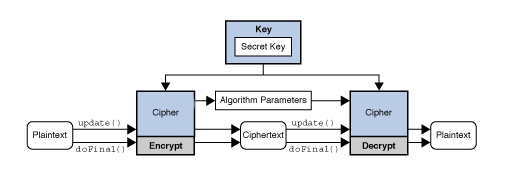
\includegraphics[scale=0.8]{./Criptografia/imagenes/cipher.png}
  \caption{Modo de uso de la clase Cipher.}
  \label{fig:cipher}
\end{figure} 

En el proyecto no hemos usado criptografía de clave simétrica, pero lo explicaremos de todas formas, ya que la forma de uso es sencilla. Se genera un objeto usando la fábrica de objetos que proporciona la clase con \lstinline{getInstance()} pasandole como parámetro una cadena con el algoritmo que queremos usar, como puede ser DES, AES, etc, junto con el padding, si es necesario, que vamos a utilizar. Un ejemplo es \lstinline{DES/CFB8/NoPadding} o \lstinline{DES/OFB32/PKCS5Padding}, acto seguido debemos de usar el procedimiento \lstinline{init()} donde debemos de indicar si el objeto se va a usar para encriptar o desencriptar y la clave usada, para finalizar podemos usar la función \lstinline{doFinal()} a la que le pasaríamos el texto cifrado o el texto en claro dependiendo del proceso que queramos usar.

Existen varias clases que heredan de la clase \lstinline{Cipher} para cifrado de flujos o de archivos enteros, sin tener que cifrar byte a byte. Por ejemplo \lstinline{CipherInputStream} y \lstinline{CipherOutputStream}. 

\textbf{Key:} para el manejo de las claves dentro del paquete hay una interfaz con la que se manejan todo tipos de claves, desde claves públicas y privadas hasta claves de cifrado simétrico. Esta interfaz la implementan un gran número de clases como pueden ser \lstinline{PrivateKey}, \lstinline{PublicKey}, \lstinline{SecretKey}, \lstinline{RSAPrivateKey}, \lstinline{RSAPublicKey}, \lstinline{DSAPrivateKey}, \lstinline{DSAPublicKey}, etc. Para generar las claves hay que usar clases factoría como pueden ser \lstinline{KeyGenerator}, \lstinline{KeyPairGenerator} o \lstinline{KeyFactory} dependiendo de si queremos generar una clave simétrica o un par de claves o usar \lstinline{KeyStore} si lo que queremos es cargar llave de un llavero (archivo de claves) que tengamos.

En el proyecto no hemos tenido que generar claves, ya que queríamos que se pudiera cargar un llavero con la clave privada y pública, en el trozo de código siguiente podemos ver como se usa la clase \lstinline{KeyStore} en el proyecto.

\begin{lstlisting}[style=Java] 
KeyStore ks = KeyStore.getInstance("PKCS12");
ks.load(new FileInputStream(path), password.toCharArray());
PrivateKey key = (PrivateKey) ks.getKey(ks.aliases().nextElement(), password.toCharArray());
\end{lstlisting}

Como podemos ver lo primero que tenemos que hacer es generar un objeto \lstinline{KeyStore}, usando la función \lstinline{getInstance()} a la que le pasaremos como parámetro el tipo de llavero que vamos a usar, nosotros hemos usado PKCS12\footnote{ Para más información visite \url{http://en.wikipedia.org/wiki/PKCS12}.}, que es un archivo creado especialmente para el almacenado de claves. Acto seguido cargamos el fichero, con el método \lstinline{load()}, al cual le pasaremos la ruta donde está el archivo físicamente y el password del archivo PKCS12. Para conseguir la clave privada usamos la función \lstinline{getKey()}, a la que hay que pasarle el alias con el que está guardada la clave en el llavero y el password. En el código se puede ver un casting, ya que la función \lstinline{getKey()} devuelve un elemento que implementa la interfaz \lstinline{Key}, pero nosotros sabemos que es un objeto de la clase \lstinline{PrivateKey}. De esta forma ya podemos usar la clave para firmar lo que necesitemos.

